\documentclass{article}
\usepackage[utf8]{inputenc}
\usepackage{authblk}
\usepackage{setspace}
\usepackage[margin=1.25in]{geometry}
\usepackage{graphicx}
\usepackage{xcolor}
\usepackage{float}
\graphicspath{ {./figures/} }
\usepackage{amsmath,amssymb,amsfonts}
\usepackage{booktabs}
\usepackage{natbib}
\usepackage{hyperref}
\hypersetup{colorlinks=true, linkcolor=blue, citecolor=blue, urlcolor=blue}

\title{\textbf{Safe Havens in Equity Crashes: Gold, Long Treasuries and Bitcoin on the Worst US Equity Days}}
\author[1]{SIQuant Research}
\affil[1]{Hypothesis $\times$ Quant}
\date{\today}
\onehalfspacing

\begin{document}
\maketitle

\begin{abstract}
\noindent \textbf{Hypothesis:} $H_0$: the mean return of the asset on the worst-decile S\&P 500 days is not positive; $H_1$: it is positive (safe haven), for gold, long Treasuries or Bitcoin \\
\textbf{Data:} daily returns of GLD, TLT and BTC-USD; crash threshold -1.10\% (10th percentile of S\&P 500 daily returns) \\
\textbf{Method:} One-sided recentred stationary bootstrap of the mean on crash days; Bonferroni $\alpha=0.0167$ for three assets \\
\textbf{Results:} GLD mean -0.10\% ($p=0.8444$); TLT mean 0.25\% ($p=0.0108$); BTC-USD mean -1.72\% ($p=1.0000$). \\
\textbf{Research decision:} \colorbox[rgb]{0.10,0.50,0.20}{\textcolor{white}{\textbf{\,ACCEPTED\,}}}
\end{abstract}

\section{Design}
A safe haven is an asset that is uncorrelated or negatively correlated with equities in market stress \citep{baur2010gold}. Crash days are defined by the 10th percentile of the whole-sample S\&P 500 return distribution, which is fixed before looking at the assets.

\section{Results}
\begin{table}[H]
\centering
\caption{Mean asset return on the worst 10\% of S\&P 500 days}
\begin{tabular}{lcccc}
\toprule
Asset & Crash days & Mean (crash) & Mean (all days) & One-sided $p$ \\
\midrule
GLD & 252 & -0.104\% & 0.050\% & 0.8444 \\
TLT & 252 & 0.254\% & -0.015\% & 0.0108 \\
BTC-USD & 252 & -1.718\% & 0.193\% & 1.0000 \\
\bottomrule
\end{tabular}
\end{table}


\begin{figure}[H]
\centering
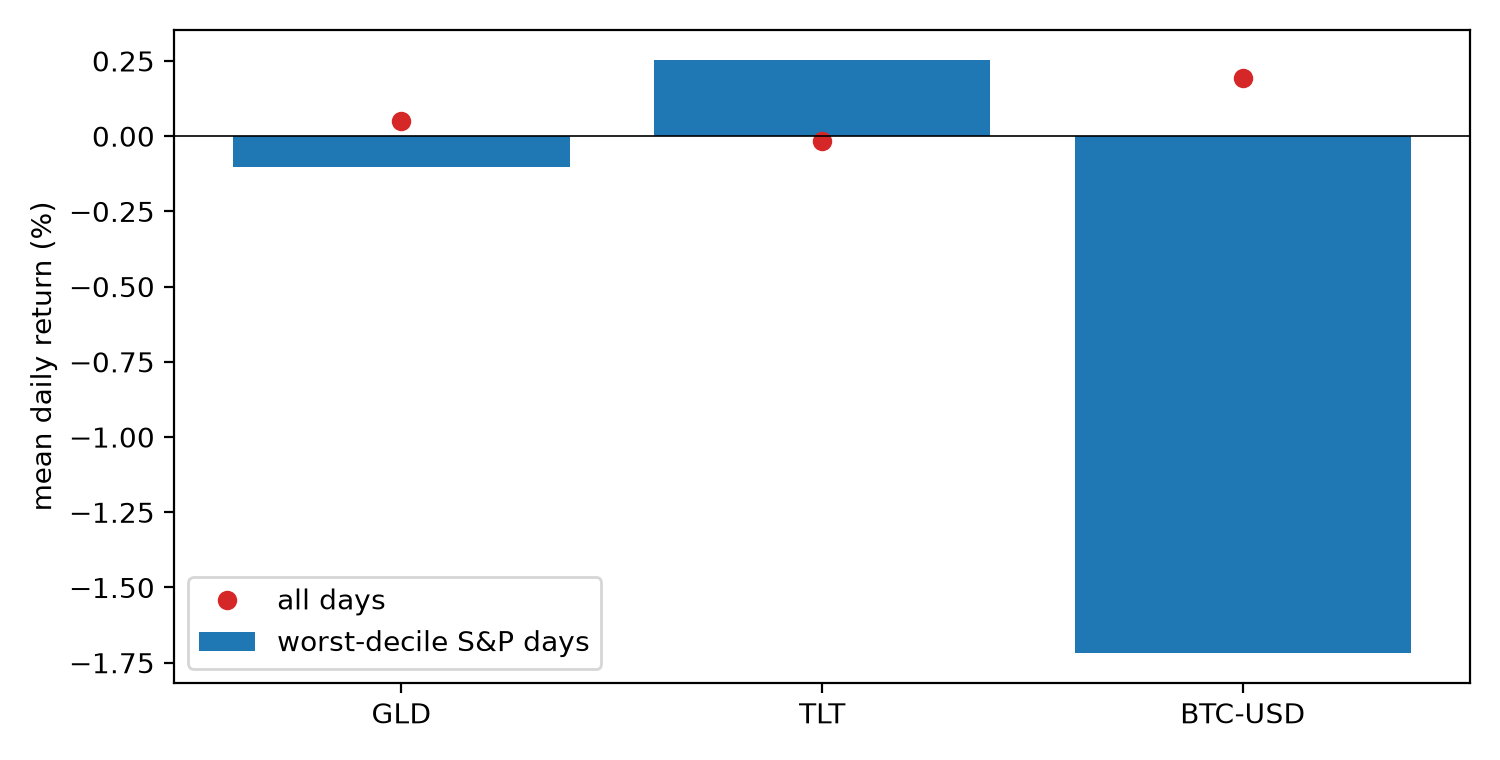
\includegraphics[width=0.8\textwidth]{fig1_safe_haven_returns.png}
\caption{Mean daily return on crash days versus all days.}
\end{figure}

\section{Limitations}
Bitcoin trades around the clock and its daily close (00:00 UTC) is not synchronous with the US close, which can blur the same-day relation. The crash days cluster in a few episodes (2018, 2020, 2022), so the effective number of independent crashes is small.


\bibliographystyle{plainnat}
\bibliography{references}

\end{document}
